\documentclass{article}
\usepackage[utf8]{inputenc}
\usepackage{graphicx}
\usepackage{ragged2e}
\usepackage{float}
\usepackage{listings}
\usepackage{xcolor}
\usepackage[spanish]{babel}
\title{kd tree}
\author{Eduardo Antonio Sanchez}
\date{Septiembre 2020}
\justifying


\begin{document}

\lstdefinestyle{customasm}{
  belowcaptionskip=1\baselineskip,
  frame=L,
  xleftmargin=\parindent,
  language=JavaScript,
  basicstyle=\footnotesize\ttfamily,
  commentstyle=\itshape\color{purple!40!black},
}

\lstdefinestyle{customc}{
  belowcaptionskip=1\baselineskip,
  breaklines=true,
  frame=L,
  xleftmargin=\parindent,
  language=JavaScript,
   basicstyle=\footnotesize\ttfamily,
  showstringspaces=false,
  basicstyle=\footnotesize\ttfamily,
  keywordstyle=\bfseries\color{green!40!black},
  commentstyle=\itshape\color{purple!40!black},
  identifierstyle=\color{blue},
  stringstyle=\color{orange},
  frame=single,   
  numbers=left,
   numberstyle=\footnotesize,
}

\lstset{escapechar=@,style=customc}

\thispagestyle{empty}

\vfill
 \begin{center}
    \begin{figure}[h]
    \centering
    \includegraphics[width=12cm]{unsa}\\
    
    \end{figure}
     
     \vspace*{1.5cm}
    {\large\bfseries FACULTAD DE PRODUCCIÓN Y SERVICIOS} \\
    {\large\bfseries ESCUELA PROFESIONAL DE CIENCIA DE LA COMPUTACIÓN}  \\ 
    
    \vspace*{1 cm}
      {\large\bfseries Práctica 1  }
       \vspace*{0.5 cm}
      
    
    \rule[0.5ex]{\linewidth}{2pt}\vspace*{-\baselineskip}\vspace*       {3.2pt}
    \rule[0.5ex]{\linewidth}{1pt}\\[\baselineskip]
    {\huge Física Computacional} \\[4mm]
    \rule[0.5ex]{\linewidth}{1pt}\vspace*{-                         \baselineskip}\vspace{3.2pt}
    \rule[0.5ex]{\linewidth}{2pt}\\
  \vspace*{1 cm}

    \begin{large}
    \bfseries DOCENTE: \\
    \bfseries Edwin Agapito Llamoca Requena  \\
     \vspace{5mm}
    \bfseries ALUMNO:\\
    \bfseries Eduardo Antonio Sanchez Hincho \\
   
   
    \end{large}
    \vspace*{0.4in}
    \noindent \\
    
    \vfill
    \large\bfseries{ AREQUIPA\\2020}
\end{center}
\newpage


\begin{flushleft}
  

\section{EJERCICIOS}

\subsection{Velocidad constante en una dimensión}
\begin{enumerate}
    \item Sea una partícula, cuya posición inicial es $t_0 = 0$, $x_0 = -5 m$,con $v_x =2 m/s$. Determine la posición de la partícula para t= 10 . Qué dirección toma?\\
    
    Este ejercicio se hizo de la siguiente forma:
     \begin{lstlisting}[language=Python,caption=Ejercicio 1]
 import matplotlib.pyplot as plt
 import numpy as np
 h=0.01
 x=-5
 vx=2
 ax=0
 px=[]
 pv=[]
 pa=[]
 pt = np.arange(0,10,h)
 for t in pt:
    x=x+vx*h
    vx=vx+ax*h
    px.append(x)
    pv.append(vx)
    pa.append(ax)

     \end{lstlisting}
    
    \begin{figure}[H]
    \centering
    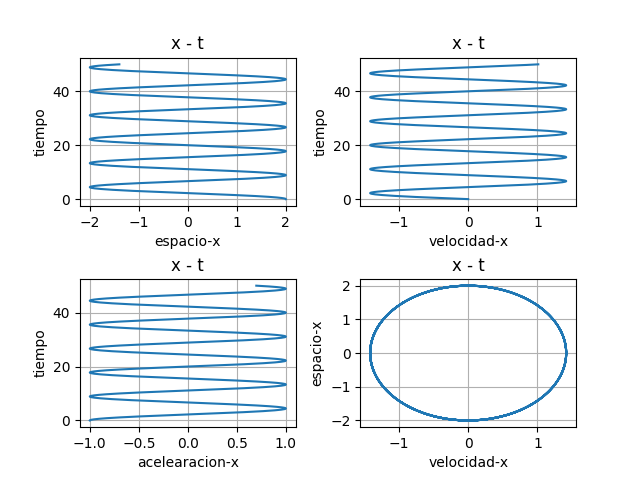
\includegraphics[width=1.21\textwidth]{Figure_1.png}
    \caption{Resultado}
    \end{figure}
        
        
    \item  Sea una partícula, cuya posición inicial es $t_0$ = 0, y = 7 m con vy = 1 m/s. A su vez se manifiesta una velocidad del viento v = −3 m/s en la dirección y. Determine la posición de la partícula para t = 10 s. Qué dirección toma? 
    \\
    En este caso nuestro código quedaría de la siguiente forma.
    \begin{lstlisting}[language=Python,caption=Ejercicio 2]
import matplotlib.pyplot as plt
import numpy as np
h=0.01
x=7
vx=-2
ax=0
px=[]
pv=[]
pa=[]
pt = np.arange(0,10,h)

for t in pt:
    x=x+vx*h
    vx=vx+ax*h
    px.append(x)
    pv.append(vx)
    pa.append(ax)
    \end{lstlisting}
    
    \begin{figure}[H]
    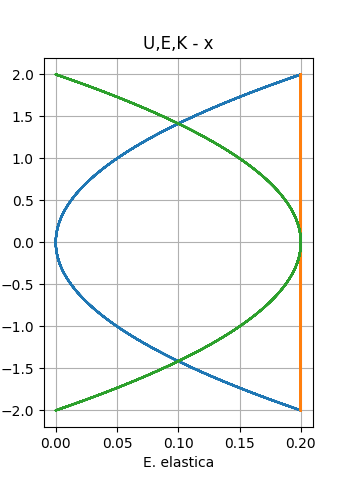
\includegraphics[width=1.3\textwidth]{Figure_2.png}
    \caption{Resultado}
    \end{figure}
    
    
    \item La posición inicial de una partícula se ubica en $x_0$ = −5 m para $t_0$ = 0 con velocidad vx = 3 m/s. Después de 3 s, se adiciona una velocidad v1 = 3 m/s transcurriendo 5 s. Después nuevamente adquiere vx = 3 m/s por 2 s. Finalmente se adiciona una velocidad de $v_2$ = −5 m/s y la partícula avanza por 5 s. Encuentre la posición de la partícula.
    
    \begin{lstlisting}[language=Python,caption=Ejercicio 3]
import matplotlib.pyplot as plt
import numpy as np
h=0.01
x=-5
vx=3
ax=0
px=[]
pv=[]
pa=[]
pt = np.arange(0,15,h)

for t in pt:
    if (t>=3 and t<8):
        vx=6
    if(t>=8 and t<10):
        vx=3
    if t>=10:
        vx=-2
    x=x+vx*h
    vx=vx+ax*h
    px.append(x)
    pv.append(vx)
    pa.append(ax)
     \end{lstlisting}
     
     \begin{figure}[H]
    \centering
    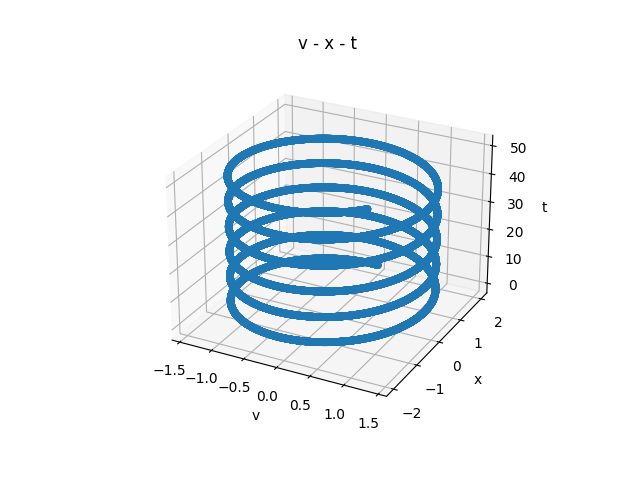
\includegraphics[width=1.4\textwidth]{Figure_3.png}
    \caption{Resultado}
    \end{figure}
    
    \item Una partícula llega a una posición final $x_0$ = 2 m en 10 s con vx = 4 m/s. Encuentre la posición
inicial cuando $t_0$= 0.\\
    El código para ello sería el siguiente.
    \begin{lstlisting}[language=Python,caption=Ejercicio 4]
import matplotlib.pyplot as plt
import numpy as np
h=0.01
x=2
vx=4
ax=0
px=[]
pv=[]
pa=[]
pt = np.arange(10,0,-h)

for t in pt:
    x=x-vx*h
    vx=vx-ax*h
    px.append(x)
    pv.append(vx)
    pa.append(ax)
        
    \end{lstlisting}
    
    \begin{figure}[H]
    \centering
    \includegraphics[width=1.4\textwidth]{Figure_4.png}
    \caption{Resultado}
    \end{figure}
    
    Si imprimimos el último elemento de nuestro lista, nos dará la distancia en el tiempo 0
    
      \begin{figure}[H]
    \centering
    \includegraphics[width=0.6\textwidth]{posicion.png}
    \caption{Posición final}
    \end{figure}
    
    \item  Un automóvil parte del reposo desde $x_0$ = 0 y pasa por x = 300 m en 2 s. Determine la velocidad.\\
    \begin{lstlisting}[language=Python,caption=Ejercicio 4]
import matplotlib.pyplot as plt
import numpy as np
h=0.01
x=0
vx=0
ax=0

pt = np.arange(0,2,h)
while x!=300:
    x=0
    vx=vx+1
    px=[]
    pv=[]
    pa=[]
    for t in pt:
        x=x+vx*h
        vx=vx+ax*h
        px.append(x)
        pv.append(vx)
        pa.append(ax)
    \end{lstlisting}
    
     \begin{figure}[H]
    \centering
    \includegraphics[width=1.35\textwidth]{Figure_5.png}
    \caption{Resultado}
    \end{figure}
    
    Respuesta: 150 m/s.
    
    \subsection{Velocidad constante en dos dimensiones}
 
        \item Una partícula parte del reposo $\vec{r}$= $(3\vec{i}+4\vec{j})$ m con una velocidad  $\vec{v}=-2\vec{i} $ m/s . Encuentre la posición final y el desplazamiento cuando t = 5 s.
        
         \begin{lstlisting}[language=Python,caption=Ejercicio 1]
 import matplotlib.pyplot as plt
 import numpy as np
 h=0.01
 x=3
 y=4
 vx=-2
 vy=0
 ax=0
 ay=0
 pt = np.arange(0,5,h)
 px=[]
 py=[]
 pv=[]
    
 pa=[]
 for t in pt:
    x=x+vx*h
    y=y+vy*h
    vx=vx+ax*h
    vy=vy+ay*h
    px.append(x)
    py.append(y)
    pv.append([vx,vy])
    pa.append([ax,ay])      
                     
          \end{lstlisting}
       
     

    \begin{figure}[H]
    \centering
    \includegraphics[width=1.35\textwidth]{Figure_6.png}
    \caption{Resultado}
    \end{figure}
    
    \item Una partícula parte del reposo $\vec{r}$= $(-3\vec{i}-4\vec{j})$ m con una velocidad  $\vec{v}=(2\vec{i} + 4\vec{j}) $ m/s . Encuentre la posición final y el desplazamiento cuando t = 5 s.
    
    
    \begin{lstlisting}[language=Python,caption=Ejercicio 2]
 import matplotlib.pyplot as plt
 import numpy as np
 h=0.01
 x=-3
 y=-4
 vx=2
 vy=4
 ax=0
 ay=0
 pt = np.arange(0,5,h)
 px=[]
 py=[]
 pv=[]
    
 pa=[]
 for t in pt:
    x=x+vx*h
    y=y+vy*h
    vx=vx+ax*h
    vy=vy+ay*h
    px.append(x)
    py.append(y)
    pv.append([vx,vy])
    pa.append([ax,ay])      
                     
          \end{lstlisting}
    
    
     \begin{figure}[H]
    \centering
    \includegraphics[width=1.35\textwidth]{Figure_7.png}
    \caption{Resultado}
    \end{figure}
    
    \item  Una partícula parte del reposo $\vec{r}$= $(3\vec{i}-4\vec{j})$ m con una velocidad  $\vec{v}=(4\vec{i} - 3\vec{j}) $ m/s .Cuando inicia su movimiento se presenta una velocidad del viento $\vec{$v_v$}= (-3\vec{i} + 5\vec{j})$  m/s. Encuentre la posición final y el desplazamiento cuando t = 10 s.\\

    El código quedaría de la siguiente forma:
    
    \begin{lstlisting}[language=Python,caption=Ejercicio 3]
 import matplotlib.pyplot as plt
 import numpy as np
 h=0.01
 x=3
 y=-4
 vx=1
 vy=2
 ax=0
 ay=0
 pt = np.arange(0,10,h)
 px=[]
 py=[]
 pv=[]
    
 pa=[]
 for t in pt:
    x=x+vx*h
    y=y+vy*h
    vx=vx+ax*h
    vy=vy+ay*h
    px.append(x)
    py.append(y)
    pv.append([vx,vy])
    pa.append([ax,ay])      
                     
          \end{lstlisting}
    
    
     \begin{figure}[H]
    \centering
    \includegraphics[width=1.35\textwidth]{Figure_8.png}
    \caption{Resultado}
    \end{figure}
    
    \subsection{Velocidad constante en tres dimensiones}
    
    \begin{itemize}
        \item Una partícula llega a una posición final  $\vec{r}$= $(-3\vec{i}-4\vec{j} - 5\vec{k})$ m  en t=5 s con una velocidad  $\vec{v}=(2\vec{j} + 4\vec{k}) $ m/s . Encuentre la posición inicial cuando  $t_0$ = 0 s.
        
        \begin{lstlisting}[language=Python,caption=Ejercicio 1]
import matplotlib.pyplot as plt
import numpy as np
h=0.01
x=-3
y=-4
z=-5
vx=0
vy=2
vz=4
ax=0
ay=0
az=0
pt = np.arange(5,0,-h)
px=[]
py=[]
pz=[]
pv=[]

pa=[]
for t in pt:
    x=x-vx*h
    y=y-vy*h
    z=z-vz*h
    vx=vx-ax*h
    vy=vy-ay*h
    vz=vz-az*h
    px.append(x)
    py.append(y)
    pz.append(z)
    pv.append([vx,vy,vz])
    pa.append([ax,ay,az])
    
    \end{lstlisting}
    
    \begin{figure}[H]
    \centering
    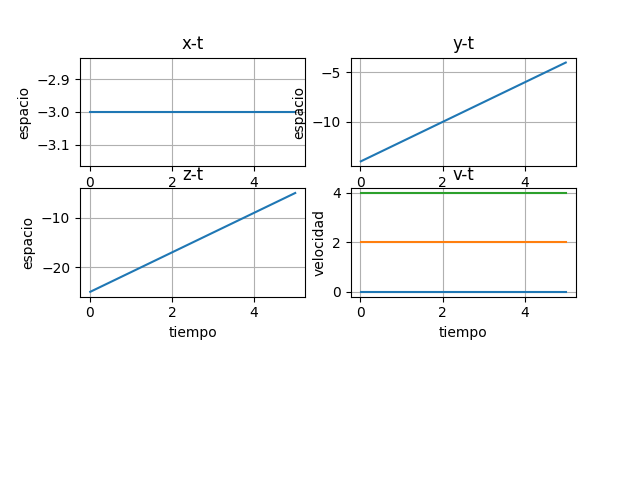
\includegraphics[width=1.3\textwidth]{3.1.png}
    \caption{Resultado}
    \end{figure}    
    
        Visto de manera 3D.
        
    \begin{figure}[H]
    \centering
    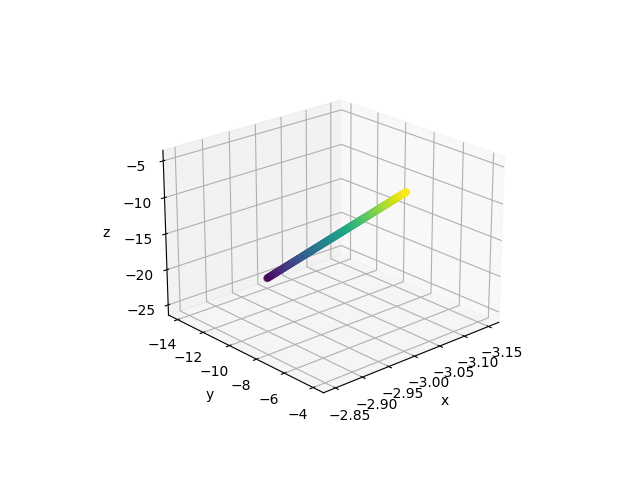
\includegraphics[width=1.35\textwidth]{3d_1.png}
    \caption{Resultado en 3D}
    \end{figure}
    
    
    
    \item Una partícula parte del reposo desde $\vec{v}$ = $(3\vec{i}- 4\vec{j} + 5\vec{k})$ m con una velocidad $\vec{v}$ = $(−2\vec{i}+ 4\vec{j} + 6\vec{k})$ m/s. Cuando inicia su movimiento se presenta una velocidad del viento $\vec{v}_v$ = $(−3\vec{j} + 5\vec{k})$ m/s.Encuentre su posición final y el desplazamiento cuando t = 10 s.
    
    \begin{lstlisting}[language=Python,caption=Ejercicio 2]
import matplotlib.pyplot as plt
import numpy as np
h=0.01
x=3
y=-4
z=5
vx=-5
vy=0
vz=11
ax=0
ay=0
az=0
pt = np.arange(0,10,h)
px=[]
py=[]
pz=[]
pv=[]

pa=[]
for t in pt:
    x=x+vx*h
    y=y+vy*h
    z=z+vz*h
    vx=vx+ax*h
    vy=vy+ay*h
    vz=vz+az*h
    px.append(x)
    py.append(y)
    pz.append(z)
    pv.append([vx,vy,vz])
    pa.append([ax,ay,az])
    
    \end{lstlisting}
    
    
    \begin{figure}[H]
    \centering
    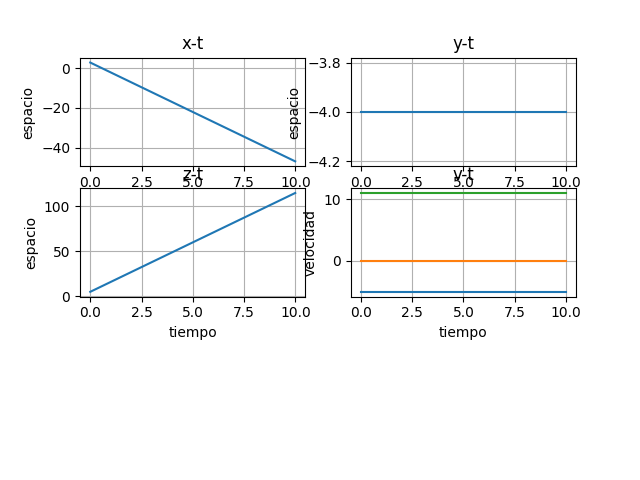
\includegraphics[width=1.2\textwidth]{3.2.png}
    \caption{Resultado}
    \end{figure}
    
    Visto de manera 3D
    
    \begin{figure}[H]
    \centering
    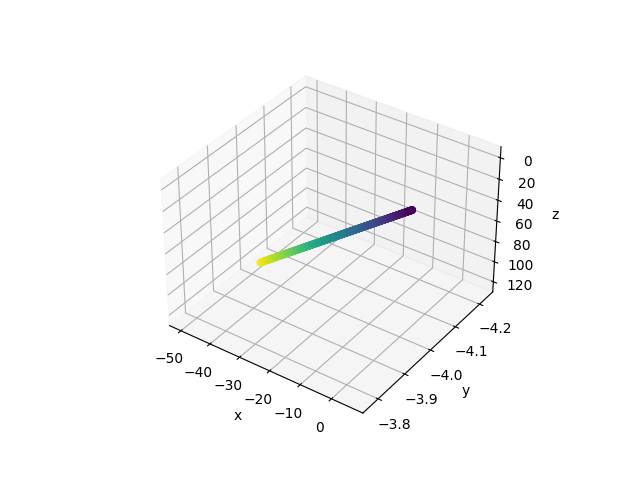
\includegraphics[width=1.35\textwidth]{3d_2.png}
    \caption{Resultado en 3D}
    \end{figure}
    
    \end{itemize}
    
    \subsection{Desafío}
    \begin{itemize}
        \item Sea un rectángulo cuyos vértices son (0, 0), (0, 10) m, (20, 0) m, (20, 10) m. Una partícula parte de
la posición inicial ubicada en (0, 0) con una velocidad ~v = (~i + 4~j) m/s. Cuando llega la partícula a
cualquier lado del rectángulo se efectúa una reflexión especular y dicha partícula continua moviéndose.
Se requiere hacer la trayectoria de la partícula para tiempos largos.
    \end{itemize}
   
     \begin{lstlisting}[language=Python,caption=Ejercicio 3]
import numpy as np
import matplotlib.pyplot as plt
import matplotlib.animation as animation

fig, ax = plt.subplots()

plt.xlim(0,20)
plt.ylim(0,10)

h=0.01

redDot, = plt.plot([0], [0], 'ro')
x=0
y=0
vx=1
vy=4


graficar, = plt.plot([], [])
x_datos, y_datos=[],[]

def animate(i):
    global x,y,vx,vy

    x_datos.append(x)
    y_datos.append(y)
    graficar.set_data(x_datos, y_datos)

    x=x+vx*h
    y=y+vy*h
    redDot.set_data(x, y)
    if(y>=10 or y<=0):
        vy=vy*-1
    if(x>=20 or x<=0):
        vx=vx*-1

    
    return redDot, graficar,


# create animation using the animate() function
myAnimation = animation.FuncAnimation(fig, animate, frames=np.arange(0,100,h), \
                                      interval=5, blit=True, repeat=False)

myAnimation.save('animation.mp4', writer='ffmpeg', fps=60);

plt.show()

     
                     
          \end{lstlisting}
   
    Se adjunta a la tarea un gif del resultado. El tiempo que se le puso para que la partícula recorra un espacio es de 100s.

\end{enumerate}
    


\end{flushleft}
\end{document}
